\title{Casper the Friendly Finality Gadget}
\author{
%        Vitalik Buterin \\
        Vitalik Buterin \textnormal{ and } Virgil Griffith \\        
        Ethereum Foundation}

\documentclass[12pt]{article}

% My goal is for the majority of Ethereum-related papers we publish use this "eth_header" template.
% make in NIPS format
\usepackage{nips10submit_e}
\nipsfinalcopy



\usepackage{graphicx}
\DeclareGraphicsExtensions{.pdf,.eps,.png,.jpg}		% search for .pdf, then .eps, then .pngs, then .jpg

% look in these subdirectories for graphics referenced by \includegraphics
% each entry must end with a /
\graphicspath{{figs/}{figures/}{images/}{./}}

\newcommand*{\red}[1]{ \color{red} #1}

\usepackage{tabularx}
\usepackage{url}
\usepackage{cite}
\usepackage{amsmath}

% for some math symbols.  Particularly \centerdot
\usepackage{ amssymb }


%\usepackage{ lmodern }			% I prefer this over times

\usepackage{array}			% replacement for eqnarray.  Must be BEFORE \usepackage{arydshln}
\usepackage{units}			% for \nicefrac{\alpha}{\beta}


\usepackage{amsthm}		% for theorems
\newtheorem{definition}{Definition}

%\usepackage{microtype}

%\usepackage{wasysym}

\usepackage{textcomp, marvosym} % pretty symbols
\usepackage{booktabs} 	% for much better looking tables

% for indicator functions
\usepackage{dsfont}

% For automatic capitalizaton of section names, etc.
\usepackage{titlesec,titlecaps}


\Addlcwords{is with of the and in}
%\Addlcwords{of the}
%\Addlcwords{and}
\titleformat{\section}[block]{}{\normalfont\Large\bfseries\thesection.\;}{0pt}{\formatsectiontitle}
\newcommand{\formatsectiontitle}[1]{\normalfont\Large\bfseries\titlecap{#1}}

\titleformat{\subsection}[block]{}{\normalfont\large\bfseries\thesubsection.\;}{0pt}{\formatsubsectiontitle}
\newcommand{\formatsubsectiontitle}[1]{\normalfont\large\bfseries\titlecap{#1}}





% for pretty Euler script
\usepackage[mathscr]{euscript}
\usepackage{bold-extra}



\usepackage{fullpage} % save trees

\usepackage{subfig}
%\usepackage{float} % for \subfloat

%%%%%%%%%%%%%%%%%%%%%%%%%%%%%%%%%%%%%%%%%%
%% More customizable Lists
%%%%%%%%%%%%%%%%%%%%%%%%%%%%%%%%%%%%%%%%%%
% Better symbols custom enumerative lists, define any symbol you'd like
\usepackage{enumitem}


%%%%%%%%%%%%%%%%%%%%%%%%%%%%%%%%%%%%%%%%%%
%% Custom Symbols 
%%%%%%%%%%%%%%%%%%%%%%%%%%%%%%%%%%%%%%%%%%
% \xspace at the end of custom macros never fucks up spacing.
% example of best practice: \newcommand{\apples}{\textsf{AppLeS}\xspace} 
\usepackage{xspace}



%%%%%%%%%%%%%%%%%%%%%%%%%%%%%%%%%%%%%%%%
%% Abbreviations you'll always want
%%%%%%%%%%%%%%%%%%%%%%%%%%%%%%%%%%%%%%%%
\newcommand*{\TODO}[1]{{\centering {\sffamily \color{red} #1} \vskip10pt }}
\newcommand*{\todo}[1]{{\sffamily [{\color{red} #1}]}}
\newcommand*{\fix}[1]{{\sffamily [{\textnormal{\color{red} #1}}]}}



%-----------------------------------------------------------------------------
%  Cross references
%-----------------------------------------------------------------------------
% The following code defines how you make references to figures, tables, etc...
% It is defined in one place only, and can be modified for all references
% in the document at the same time.
% Instead of typing each time: "see Fig. \ref{myfig}" you can create a command
% \figref which will do the job. Then in text you only type \figref{myfig} and LaTeX
% will do the rest.
\newcommand{\tblref}[1]{Table~\ref{#1}}
%\renewcommand*{\figref}[1]{Fig.~\ref{#1}}
\renewcommand{\eqref}[1]{eq.~\ref{#1}}


\newcommand{\figref}[1]{Figure~\ref{#1}}
\newcommand{\Figref}[1]{Figure~\ref{#1}}
\newtheorem{theorem}{Theorem}
\newtheorem{lemma}[theorem]{Lemma}

%%%%%%%%%%%%%%%%%%%%%%%%%%%%%%%%%%%%%%%%

% for \sout{} for strikeout
\usepackage[normalem]{ulem}


% for better manipulation of tables
\usepackage{makecell}
\renewcommand\theadfont{\bfseries}


%-----------------------------------------------------------------------------
%  Misc symbols that I like
%-----------------------------------------------------------------------------
\newcommand*{\opname}[1]{\operatorname{#1}}


\renewcommand*{\to}{\rightarrow}


%%%%





%\usepackage{mathenv}
%\usepackage[]{algorithm2e}
\usepackage{listings}


%% Special symbols we'll probably iterate on
%%%%%%%%%%%%%%%%%%%%%%%%%%%%%%%%%%%%%%%%%%%%%%%%%%%%%%
% we will probably iterate on these symbols until we have a notation we like
\newcommand{\epoch}{\ensuremath{e}\xspace}
\newcommand{\hash}{\ensuremath{c}\xspace}

% symbols for the epoch and hash source
\newcommand{\epochsource}{\ensuremath{\overset{\to}{\epoch}}\space}
\newcommand{\hashsource}{\ensuremath{\overset{\to}{\hash}}\xspace}

\newcommand{\signature}{\ensuremath{\mathcal{S}}\xspace}

\newcommand{\totaldeposit}{\textnormal{TD}\xspace}

\newcommand{\gamesymbol}{\reflectbox{G}}

\newcommand{\msgPREPARE}{\textbf{\textsc{prepare}}\xspace}
\newcommand{\msgCOMMIT}{\textbf{\textsc{commit}}\xspace}

% Symbols for the Last Justified Epoch and Hash
\newcommand{\epochLJ}{\ensuremath{\epoch_{\textnormal{LJ}}}\xspace}
\newcommand{\hashLJ}{\ensuremath{\hash_{\textnormal{LJ}}}\space}

% Symbols for the Last Finalized Epoch and Hash
\newcommand{\epochLF}{\ensuremath{\epoch_{\textnormal{LF}}}\xspace}
\newcommand{\hashLF}{\ensuremath{\hash_{\textnormal{LF}}}\space}

% Griefing Factor symbol
\newcommand{\GF}[1]{\mathds{GF}\left( #1 \right)\xspace}

% Genesis block symbol
\newcommand{\Genesisblock}{\ensuremath{G}\xspace}


\begin{document}

\maketitle

%%%%%%%%%%%%%%%%%%%%%%%%%%%%%%%%%%%%%%%%%%%%%%%%%%%%%%%%%%%%%%%%%%%%%%%%%%%%%%%%%%%%%%%%%%%%%%%%%%%%%%%%%%%%%%%%%%%%%%%%%%
%%%%%%%%%%%%%%%%%%%%%%%%%%%%%%%%%%%%%%%%%%%%%%%%%%%%%%%%%%%%%%%%%%%%%%%%%%%%%%%%%%%%%%%%%%%%%%%%%%%%%%%%%%%%%%%%%%%%%%%%%%

\begin{abstract}
We give an introduction to the consensus algorithm details of Casper: the Friendly Finality Gadget, as an overlay on an existing proof of work blockchain such as Ethereum. Casper is a partial consensus mechanism inspired by a combination of existing proof of stake algorithm research and Byzantine fault tolerant consensus theory, which if overlaid onto another blockchain (which could theoretically be proof of work or proof of stake) adds strong \textit{finality} guarantees that improve the blockchain's resistance to transaction reversion (or ``double spend'') attacks.
\end{abstract}

%%%%%%%%%%%%%%%%%%%%%%%%%%%%%%%%%%%%%%%%%%%%%%%%%%%%%%%%%%%%%%%%%%%%%%%%%%%%%%%%%%%%%%%%%%%%%%%%%%%%%%%%%%%%%%%%%%%%%%%%%%
%%%%%%%%%%%%%%%%%%%%%%%%%%%%%%%%%%%%%%%%%%%%%%%%%%%%%%%%%%%%%%%%%%%%%%%%%%%%%%%%%%%%%%%%%%%%%%%%%%%%%%%%%%%%%%%%%%%%%%%%%%
\section{Introduction}
\label{sect:intro}

The past few years there has been considerable research into ``proof of stake'' (PoS) based blockchain consensus algorithms. In a PoS system, a blockchain appends and agrees on new blocks through a process where anyone who holds coins inside of the system can participate, and the influence someone has is proportional to the number of coins (or ``stake'') they hold. This is a vastly more efficient alternative to proof of work ``mining'', allowing blockchains to operate without mining's high hardware and electricity costs.

There are two major schools of thought in PoS design. The first, \textit{chain-based proof of stake}, mimics proof of work mechanics featuring a chain of blocks and an algorithm that ``simulates'' mining by pseudorandomly assigning the right to create new blocks to stakeholders.  This includes Peercoin \cite{king2012ppcoin}, Blackcoin\cite{vasin2014blackcoin}, and Iddo Bentov's work\cite{bentov2016pos}.

The other school, \textit{Byzantine fault tolerant} (BFT) based proof of stake, is based on a thirty year old body of research into BFT consensus algorithms such as PBFT\cite{castro1999practical}. BFT algorithms typically have proven mathematical properties; for example, one can usually mathematically prove that as long as $>\frac{2}{3}$ of protocol participants are following the protocol honestly, then, regardless of network latency, the algorithm cannot finalize conflicting block hashes (called ``safety'').  Repurposing BFT algorithms for proof of stake was first introduced by Tendermint\cite{kwon2014tendermint}.

\subsection{Our Work}
We follow the BFT tradition, though with some modifications. Casper the Friendly Finality Gadget is an \textit{overlay} atop a \textit{proposal mechanism}---a mechanism which proposes \textit{checkpoints}.  Casper is responsible for \textit{finalizing} these checkpoints.  Casper provides safety, but does not guarantee liveness---Casper depends on the proposal mechanism for liveness.  That is, even if the proposal mechanism is wholly controlled by attackers, Casper prevents attackers from finalizing two conflicting checkpoints, however, the attackers can prevent Casper from finalizing any future checkpoints.


Our algorithm introduces several new properties that BFT algorithms do not necessarily support.
\begin{itemize}
\item We flip the emphasis of the proof statement from the traditional ``as long as $>\frac{2}{3}$ of validators are honest, there will be no safety failures'' to the contrapositive ``if there is a safety failure, then $\ge \frac{1}{3}$ of validators violated some protocol rule.''

\item We add \textit{accountability}.  If a validator violates the rules, we can detect the violation, and know who violated the rule.  ``$\ge \frac{1}{3}$ violated the rules, \textit{and we know who they are}''.  Accountability allows us to penalize malfeasant validators, solving the \textit{nothing at stake} problem \todo{cite} that plagues chain-based PoS. The penalty is the validators' entire deposits.  This maximum penalty is provides a bulwark against violating the protocol by making violations immensely expensive.  Protocol guarantees is much higher than the size of the rewards that the system pays out during normal operation.  This provides \textit{stronger} security guarantees than with proof of work.

\item We introduce a provably safe way for the validator set to change over time (Section \ref{sect:join_and_leave}).
\item We introduce a way to recover from attacks where more than $\frac{1}{3}$ of validators drop offline, at the cost of a very weak \textit{tradeoff synchronicity assumption} (Section \ref{sect:leak}).
\item The design of the algorithm as an overlay makes it easier to implement as an upgrade to an existing proof of work chain.
\end{itemize}

We will describe the protocol in stages, starting with a simple version (Section \ref{sect:protocol}) and then progressively adding features such as validator set changes (Section \ref{sect:join_and_leave}) and mass liveness fault recovery (Section \ref{sect:leak}). 

%%%%%%%%%%%%%%%%%%%%%%%%%%%%%%%%%%%%%%%%%%%%%%%%%%%%%%%%%%%%%%%%%%%%%%%%%%%%%%%%%%%%%%%%%%%%%%%%%%%%%%%%%%%%%%%%%%%%%%%%%%
%%%%%%%%%%%%%%%%%%%%%%%%%%%%%%%%%%%%%%%%%%%%%%%%%%%%%%%%%%%%%%%%%%%%%%%%%%%%%%%%%%%%%%%%%%%%%%%%%%%%%%%%%%%%%%%%%%%%%%%%%%

\section{The Casper Protocol}
\label{sect:protocol}
In the simple version, we assume there is a set of validators and a \textit{proposal mechanism} which is any system that proposes a sequence of blocks (such as a proof of work chain)


We order the sequence of blockhashes into a sequence called a \emph{blockchain} $\mathbf{B}$.  We assume all blocks $b \in \mathbf{B}$ are unique.  The elements of sequence $\mathbf{B}$ obey a total ordering where $b < b^\prime$ if and only if block $b$ precedes block $b^\prime$ in within sequence $\mathbf{B}$. Within blockchain $\mathbf{B}$ is there is a subset called \emph{checkpoints},

\begin{equation}
\begin{split}
    \mathbf{B} &\equiv \left( b_0, b_1, b_2, \ldots \right) \\
    \mathbf{C} &\equiv \left( b_0, b_{99}, b_{199}, b_{299}, \ldots \right) \; .
\end{split}
\end{equation}

This leads to the formula for an arbitrary checkpoint,
\begin{equation}
    C_i = \begin{cases}
     b_0 \qquad \qquad \qquad\ \  \textnormal{if } i = 1, \\
     b_{ 100*(i-2) + 99 } \qquad \textnormal{otherwise.}
     \end{cases}
\end{equation}

The proposal mechanism will initially be the existing Ethereum proof of work chain, making the first version of Casper a \textit{hybrid PoW/PoS algorithm} that relies on proof of work for liveness but not safety, but in future versions the proposal mechanism can be substituted with something else.

An \emph{epoch} is defined as the contiguous sequence of blocks between two checkpoints.  The \textit{epoch of a block} is the index of the epoch containing that hash, e.g., the epoch of block 599 is 5.\footnote{To get the epoch of a particular block $b_i$, it is $epoch(b_i) = \lfloor i / 100 \rfloor$.}. Likewise, the epoch of checkpoint $C_n$ is simply $n - 1$.

%\begin{equation}
%    \begin{split}
%    epoch(k) &\equiv \left( b_{100k}, b_{100k + 1}, \ldots, b_{100k + 99} \right) \\
%    epoch(c) & \equiv i-1 \qquad \textnormal{such that } C_i = c
%    \end{split} \; .
%\end{equation}


Each validator has a \emph{deposit}; when a validator joins their deposit is the number of coins that they deposited, and from there on each validator's deposit rises and falls with rewards and penalties. For the rest of this paper, when we say ``$\frac{2}{3}$ of validators'', we are referring to a \emph{deposit-weighted} fraction; that is, a set of validators whose sum deposit size equals to at least $\frac{2}{3}$ of the total deposit size of the entire set of validators. ``$\frac{2}{3}$ prepares'' will be used as shorthand for ``prepares from $\frac{2}{3}$ of validators''.

Validators can broadcast two types of messages: $\left\langle \msgPREPARE, \hashsource, \epochsource, \hash, \epoch \right\rangle$ and $\left\langle \msgCOMMIT, \hash, \epoch \right\rangle$, as detailed in \figref{fig:messages}.

Every checkpoint $\hash$ can be \emph{Justified}.  Justified checkpoints can then also be \emph{Finalized}.  Every checkpoint starts as neither Justified or Finalized.


\begin{equation}
\begin{split}
    \mathbf{J} &= \left( c \in \mathbf{C} : \textnormal{valid\_prepares}(c) \geq \nicefrac{2}{3} \right) \\
    \mathbf{F} &= \left( j \in \mathbf{J} \,: \textnormal{valid\_commits}(j) \geq \nicefrac{2}{3} \right)\; .
\end{split}
\label{eq:firstJandF}
\end{equation}


%\TODO{still deciding this mathematical notation.  But it should be mathematical instead of in words.}

Which leads to the pleasing relation, $\mathbf{F} \subseteq \mathbf{J} \subseteq \mathbf{C} \subset \mathbf{B}$.



\begin{figure}[h!tb]
\centering

   \begin{subfigure}[b]{\textwidth}
   \centering
   \begin{tabular}{l l}
	\toprule
	\textbf{Notation} & \textbf{Description} \\
	\midrule
	$\hashsource$ & the hash of any Justified checkpoint \\
	$\epochsource$ & the epoch of checkpoint $\hashsource$  \\
	\hash & any checkpoint hash after $\hashsource$ \\
	$\epoch$ & the epoch of checkpoint \hash \\
	\signature & signature of $\left\langle \msgPREPARE, \hashsource,\epochsource, \hash, \epoch \right\rangle$ from the validator's private key \\
	\bottomrule
	\end{tabular}
	\caption{\msgPREPARE message}
	\label{fig:msgPREPARE}	
	\end{subfigure}

   \vspace{0.2in}


   \begin{subfigure}[b]{\textwidth}
   \centering
    \begin{tabular}{l l}
	\toprule
	\textbf{Notation} & \textbf{Description} \\
	\midrule
	\hash & a Justified checkpoint hash \\
	\epoch & the epoch of the checkpoint \hash \\
	\signature & signature of $\langle \msgCOMMIT, \epoch, \hash \rangle$ from the validator's private key \\
	\bottomrule	
	\end{tabular}
	\caption{\msgCOMMIT message}
	\label{fig:msgCOMMIT}	
	\end{subfigure}


\caption{The schematic of \msgPREPARE and \msgCOMMIT messages.}
\label{fig:messages}
\end{figure}


%A hash $\hash$ converts from fresh to \emph{Justified} if and only if $\frac{2}{3}$ of validators send prepares of the form,

%\begin{equation}
%\langle \msgPREPARE, \epoch(\hash), \hash, \epoch(\hashsource), \hashsource, \signature \rangle  \; .
%\label{eq:msgPREPAREtwo}
%\end{equation}

%for some specific $\hashsource$. A hash $\hash$ can only be Justified if its $\hashsource$ is already Justified.

\textbf{Requirements for accepting a prepare message (\figref{fig:msgPREPARE})}:
\begin{enumerate}
\item Hash \hashsource must be the checkpoint for epoch \epochsource.  $c = b_{100\epochsource + 99}$
\item Hash \hashsource must be Justified.  Equivalently, $\textnormal{valid\_prepares}(c) \geq \nicefrac{2}{3}$.
\item Hash \hash must be the checkpoint for epoch \epoch.  Equivalently, $\hash = b_{100\epoch + 99}$.
\item Epoch $\epochsource < \epoch$.
\item[5a.] The signing validator must be a member of the validator set.
\end{enumerate}
If all requirements are satisfied, then the sending validator's deposit counts as preparing $\hashsource \to \hash$.

%Additionally, a hash $\hash$ converts from Justified to \emph{Finalized}, if $\frac{2}{3}$ of validators commit

%\begin{equation}
%\langle \msgCOMMIT, \epoch(\hash), \hash \rangle \; ,
%\label{eq:msgCOMMITtwo}
%\end{equation}


\textbf{Requirements for accepting a commit message (\figref{fig:msgCOMMIT})}:
\begin{enumerate}
\item Hash \hash must be the checkpoint of epoch \epoch.  Equivalently, $\hash = b_{100\epoch + 99}$.
\item Hash \hash must be \emph{already} Justified.  Meaning checkpoint \hash must have been Justified before the commit message.  Equivalently, $c \in \mathbf{J}$.
\item Hash \hash must have been Justified within the past 100 blocks.  Equivalently, if checkpoint \hash became Justified at block $b_i$, then the commits will only be accepted between blocks $[ b_{i+1}, b_{i+101} ]$.
\item[3a.] The signing validator must be a member of the validator set.
\end{enumerate}
If all requirements are satisfied, then the sending validator's deposit counts as behind commiting checkpoint \hash.

Validators only recognize prepares and commits that have been included in blocks (even if those blocks are not part of the main chain). 

The most notable property of Casper is that it is impossible for two conflicting checkpoints to be Finalized unless $\geq \frac{1}{3}$ of the validators violated one of the two\footnote{Earlier versions of Casper had four slashing conditions \cite{minslashing}, but we can reduce to two because of the requirements that (i) Committed hashes must already be Justified, and (ii) prepare messages must point to an already Justified ancestor.  These requirements ensure that blocks will not register commits or prepares that violate the other two slashing conditions, making them superfluous.} Casper Commandments (a.k.a. slashing conditions).  These are:

\begin{enumerate}
   \item[\textbf{I.}] \textsc{A validator shalt not publish nonidentical prepares specifying the same target epoch.}

   In other words, for each epoch \epoch, a validator may prepare at most exactly one $\left(\hashsource, \epochsource, \hash\right)$ triplet.

   \item[\textbf{II.}] \textsc{A validator shalt not commit to any epoch between the epochs of its own prepare statements.}
    
   Equivalently, a validator may never publish,
\begin{equation}
\left\langle \msgPREPARE, \hashsource, \epochsource, \hash_p, \epoch_p \right\rangle \hspace{0.5in} \textnormal{and} \hspace{0.5in} \left\langle \msgCOMMIT, \epoch_c, \hash_c \right\rangle \;, 
\label{eq:msgPREPARE}
\end{equation}

where the epochs satisfy $\epochsource < \epoch_c < \epoch_p$.

\end{enumerate}

If a validator violates any commandment, the evidence that the validator did this can be included into the blockchain as a transaction, at which point the validator's entire deposit will be taken away, with a 4\% ``finder's fee'' given to the submitter of the evidence transaction.

\subsection{Casper's Fork Choice Rule}
\label{sect:forkchoice}
Casper is more complicated than standard PoW designs.  As such, the fork-choice must be adjusted.  This fork-choice rule should be followed by all users, validators, and even the underlying block proposal mechanism.  If the users, validators, or block-proposers instead follow the typical fork-choice rule of ``always build atop the longest chain'', there are pathological scenarios where Casper gets ``stuck'' and any blocks built atop the longest chain cannot be Finalized (or even Justified) without violating a Commandment---one such pathological scenario is the fork in \figref{fig:forkchoice}.

In \figref{fig:forkchoice_a}, proposers follow the ``build atop the longest chain'' rule and proposers build atop $A_2$.  But this runs into problems.  $A_2$ cannot be Justified by Preparing $A_1 \to A_2$ because that requires first Justifying $A_1$.  Unfortunately, because another block with the same epoch ($B_1$) is already Justified (has $\frac{2}{3}$ prepares), $A_1$ cannot be Justified without at least $\frac{1}{3}$ of validators violating Commandment \textbf{I} by preparing both $A_1$ and $B_1$.

Since we can't justify $A_1$, could we instead Justify $A_2$ by preparing $S \to A_2$?  Unfortunately, preparing $S \to A_2$ to Justification requires some validators to violate Commandment \textbf{II} as $\frac{1}{2}$ have already commited to $B_1$.  This same argument applies to any ancestor of $S$.  Therefore $A_2$ cannot be Justified by any means without violating a Commandment.  Then because $A_2$ cannot be Justified, it cannot be Finalized.  Even more unfortunate, this same argument also applies to all successors of $A_2$.  Ergo, if validators are Rational and follow the longest-chain fork-choice rule, \emph{no checkpoints would be justified or finalized ever again}.

Fortunately, there's another way; in \figref{fig:forkchoice_b} we see the way out.  Say we instead built atop $B_1$ to create $B_2$.  Unfortunately $B_2$ cannot be Justified because preparing $B_1 \to B_2$ to justification requires some validators to violate Commandment \textbf{I} as $\frac{1}{2}$ have already prepared to $A_2$ (and likewise cannot prepare $S \to B_2$ because $\frac{1}{2}$ have already committed to $B_1$).  So there's no way to Justify $B_2$.  Then because $B_2$ cannot be Justified, it cannot be Finalized.  But say we keep building and create $B_3$.  Validators \emph{can} prepare $B_1 \to B_3$ without violating Commandment \textbf{I}.  And secondly, because $A_2$ has no commits, all validators can prepare $B_1 \to B_3$ without violating Commandment \textbf{II}.  Once $B_3$ is Justified, it can be Finalized without obstacles.



\begin{figure}[h!tb]
\centering
   \begin{subfigure}[b]{0.42\textwidth}
   \centering
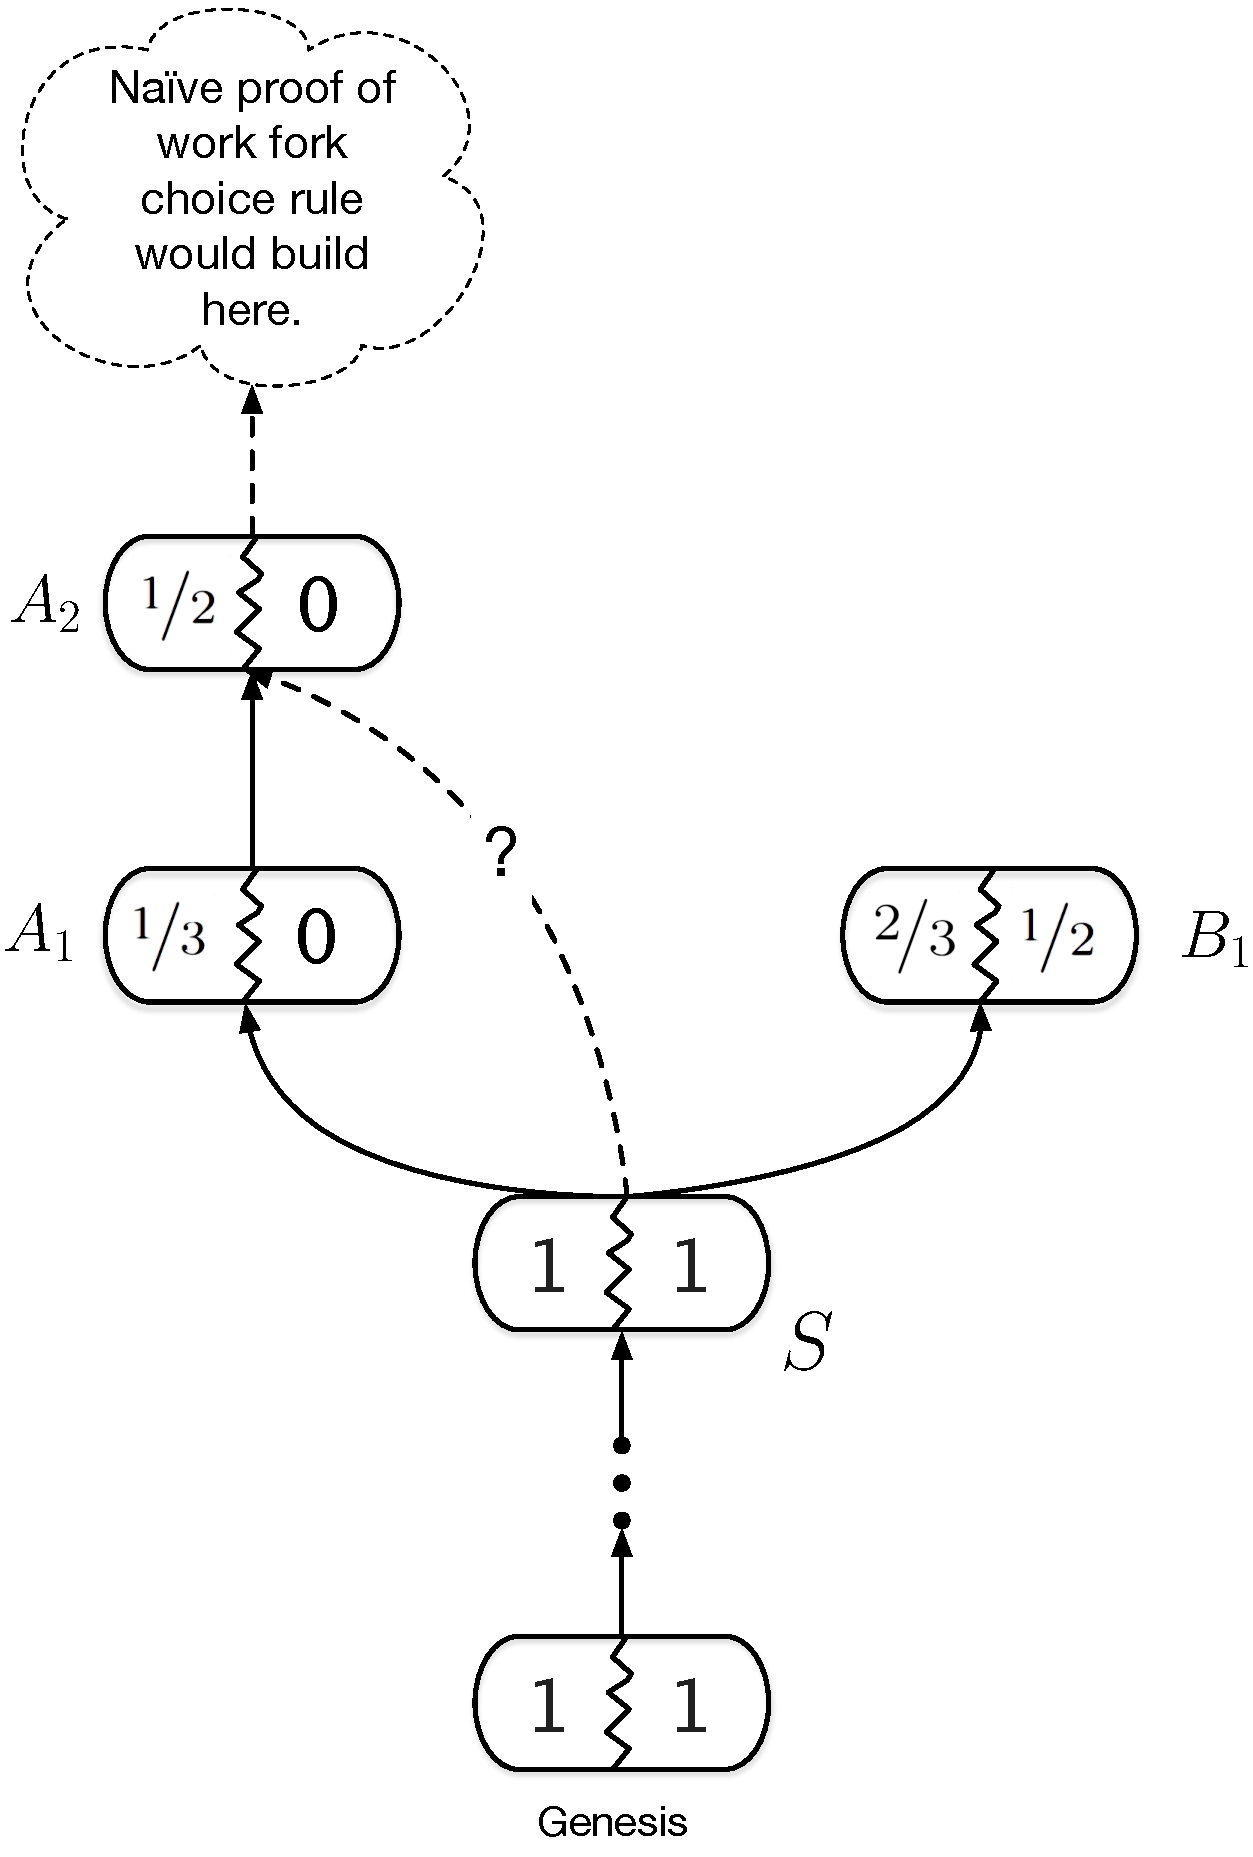
\includegraphics[width=2.5in]{forkchoiceruleA.pdf}
	\caption{Longest-chain forkchoice rule.}
	\label{fig:forkchoice_a}	
	\end{subfigure} \hspace{0.3in} \begin{subfigure}[b]{0.42\textwidth}
   \centering
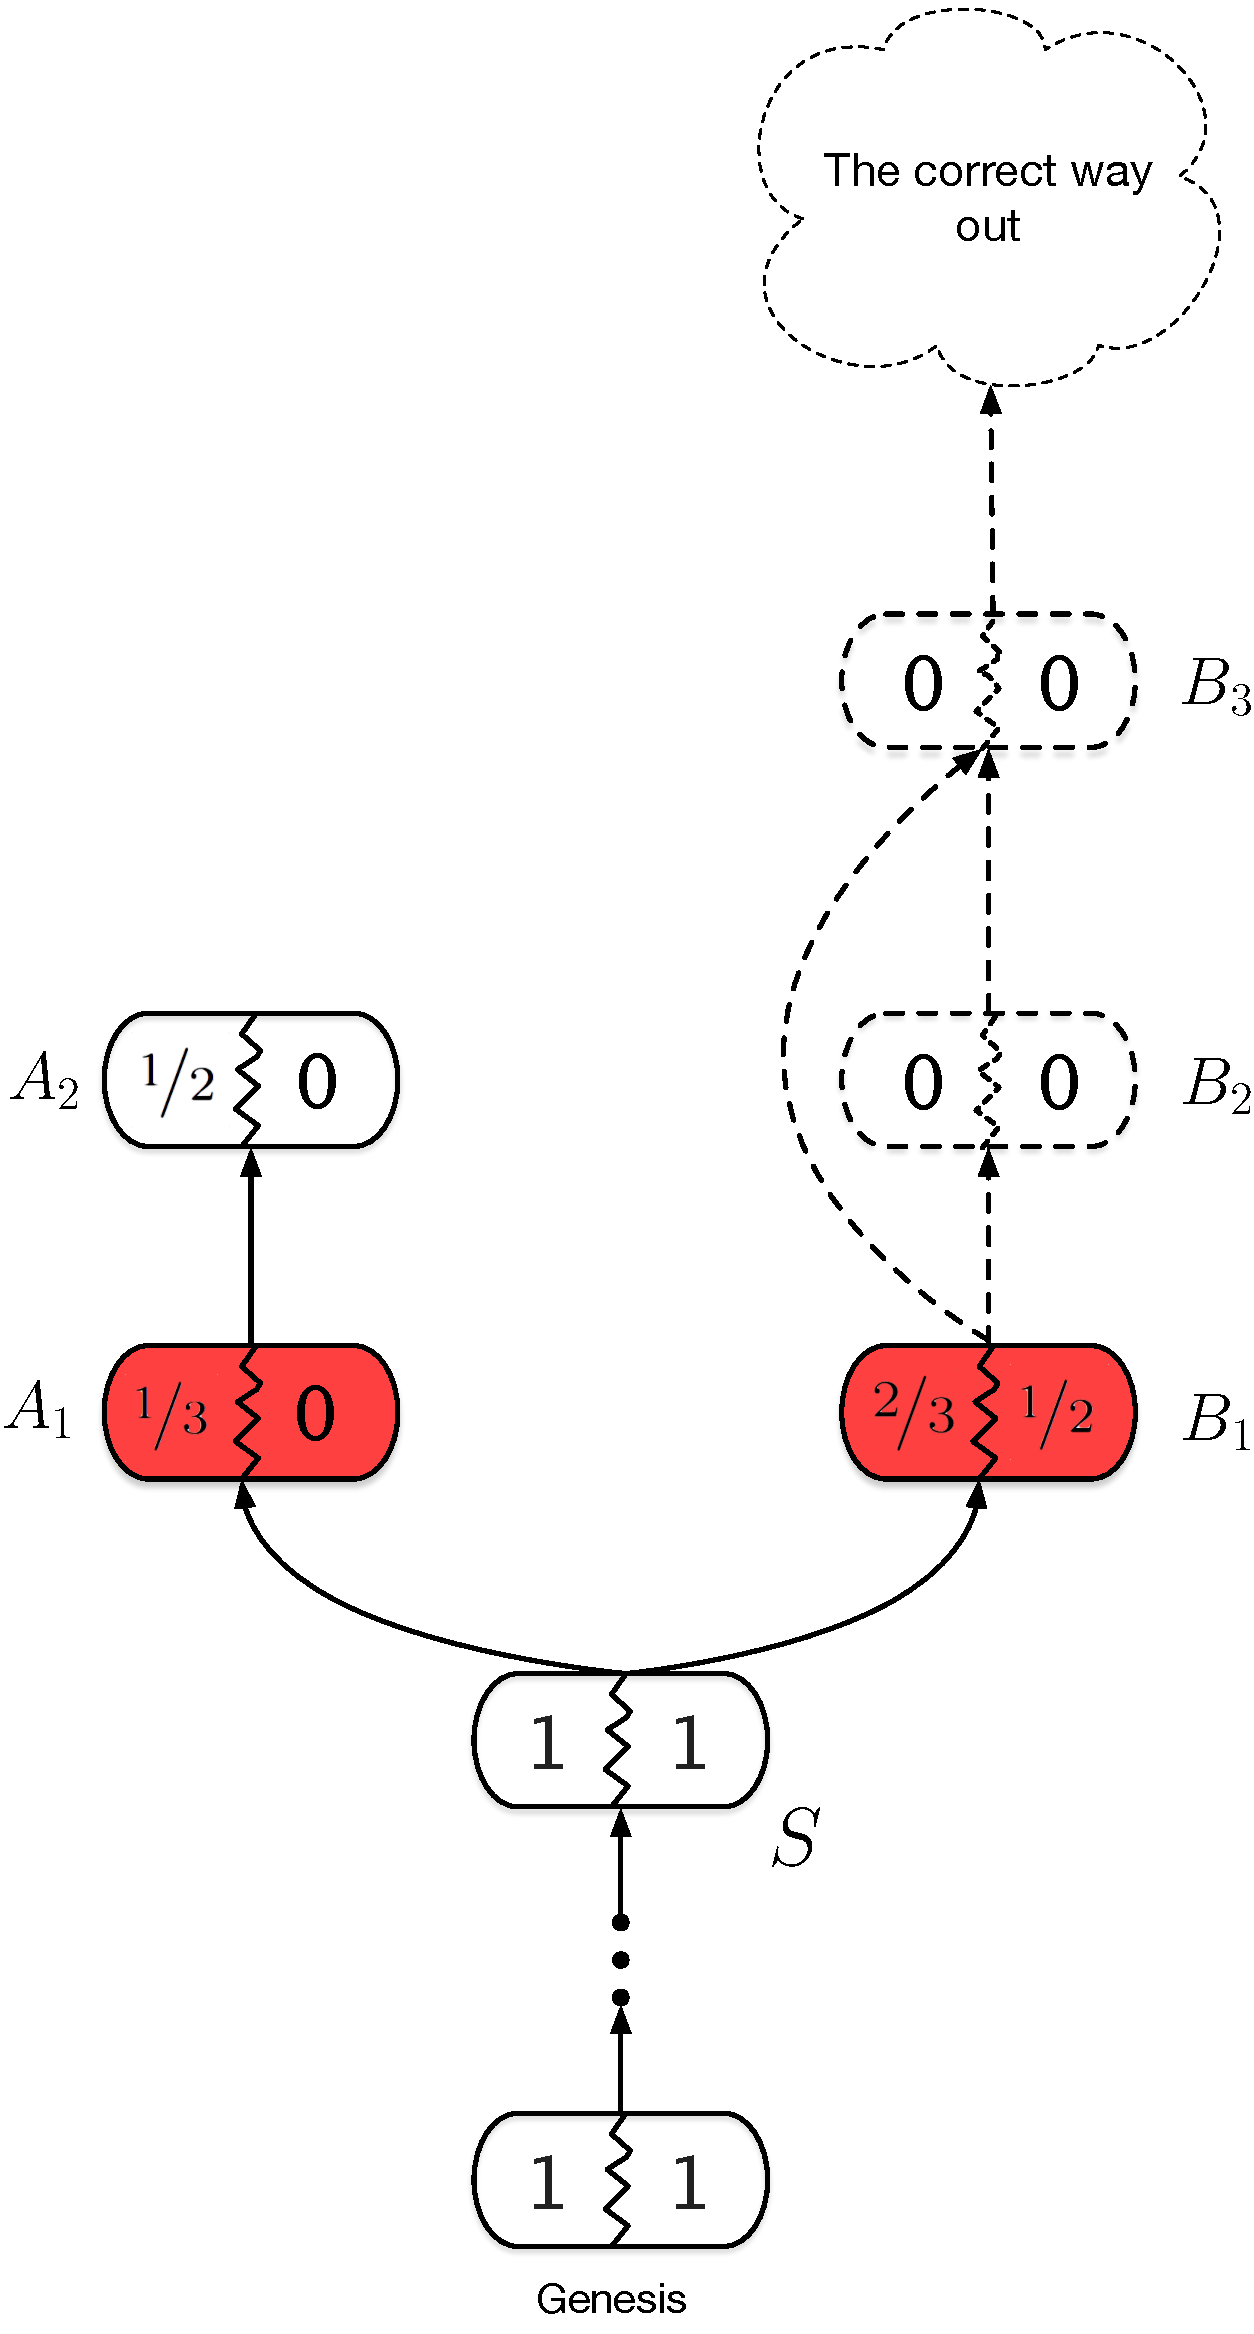
\includegraphics[width=2.5in]{forkchoiceruleB.pdf}
	\caption{Casper-aware forkchoice rule.}
	\label{fig:forkchoice_b}	
	\end{subfigure}

\caption{A pathological scenario demonstrating the outcome of two fork-choice rules.   In \Subref{fig:forkchoice_a} we see the result of the typical ``build atop the longest chain'' fork choice rule.  In \Subref{fig:forkchoice_b} we see the result of our Casper-aware fork choice rule (Listing \ref{alg:forkchoice}).  Each pill represents a checkpoint.  In each pill, the left number is the proportion of validators who prepared that checkpoint, and the right number is the proportion of validators who committed that checkpoint.  Red pills are conflicting checkpoints.}
\label{fig:forkchoice}
\end{figure}

Inspired by the successful escape in \figref{fig:forkchoice_b}, we define a novel fork choice rule.\footnote{Casper's commit-following fork choice rule is analogous to the ``greedy heaviest observed subtree'' (GHOST) rule for proof of work chains\cite{sompolinsky2013accelerating}.} Instead of blindly following the longest-chain, we:

\begin{enumerate}
\item Favor checkpoints by the proportion of commits.
\item When multiple checkpoints have the same proportion of commits, favor checkpoints by the proportion of prepares.
\item When multiple checkpoints have the same proportion of prepares, favor checkpoints by depth (longest chain).
\item When multiple checkpoints have the same depth, choose randomly.
\end{enumerate}

A complete specification for our forkchoice rule is in Listing \ref{alg:forkchoice}.  The Casper fork-choice rule ensures that the selected head will always be one that minimizes validator penalties.  In fact, as long as $> \frac{2}{3}$ of validators only commit to Justified checkpoints, there \emph{never} needs to be a violation of either Commandment (see Theorem \ref{theorem:liveness}).



%%%%%%%%%%%%%%%%%%%%%%%%%%%%%%%%%%%%%%%%%%%%%%%%%%%%%%%%%%%%%%%%%%%%%%%%%%%%%%%%%%%%%%%%%%%%%%%%%%%%%%%%%%%%%%%%%%%%%%%%%%
%%%%%%%%%%%%%%%%%%%%%%%%%%%%%%%%%%%%%%%%%%%%%%%%%%%%%%%%%%%%%%%%%%%%%%%%%%%%%%%%%%%%%%%%%%%%%%%%%%%%%%%%%%%%%%%%%%%%%%%%%%
\section{Proofs of Safety and Plausible Liveness}
\label{sect:theorems}

We prove Casper's two fundamental properties: \textit{accountable safety} and \textit{plausible liveness}. Accountable safety means that two conflicting checkpoints cannot be Finalized unless $\geq \frac{1}{3}$ of validators violate a slashing condition (meaning at least one third of the total deposit is lost).  Plausible liveness means that, regardless of any previous events, it is always possible for $\frac{2}{3}$ of honest validators to finalize a new checkpoint.

\begin{theorem}[Accountable Safety]
\label{theorem:safety}
Two conflicting checkpoints cannot be Finalized unless $\geq \frac{1}{3}$ of validators violate a slashing condition.

\begin{proof}
Suppose the two conflicting checkpoints are $A$ in epoch $\epoch_A$ and $B$ in epoch $\epoch_B$ (see \figref{fig:conflicting_checkpoints}). If both are Finalized, this entails $\frac{2}{3}$ commits and $\frac{2}{3}$ prepares in epochs $\epoch_A$ and $e_B$. In the trivial case where $\epoch_A = \epoch_B$ (\figref{fig:2a}), this implies that some intersection of $\geq \frac{1}{3}$ of validators must have violated Commandment \textbf{I}. If instead $\epoch_A \not= \epoch_B$, there exist two chains $\Genesisblock < \cdots < \epoch_A^2 < \epoch_A^1 < \epoch_A$ and $\Genesisblock < \cdots < \epoch_B^2 < \epoch_B^1 < \epoch_B$ of Justified checkpoints, both terminating at the genesis block $\Genesisblock$. Without loss of generality, suppose $\epoch_A < \epoch_B$. Then, there must be some $\epoch_B^i$ such that $\epoch_B^i \leq \epoch_A < \epoch_B$.  If $\epoch_B^i = \epoch_A$ (\figref{fig:2b}), then checkpoints $A$ and $B^i$ both have $\frac{2}{3}$ prepares, thus $\geq \frac{1}{3}$ of validators violated Commandment \textbf{I}.  If instead $\epoch_B^i < \epoch_A$ (\figref{fig:2c}), checkpoint $A$ has at least $\frac{2}{3}$ commits and checkpoint $\epoch_B^i$ has at least $\frac{2}{3}$ prepares with $\epoch_B^i < \epoch_A < \epoch_B$.  Therefore $\geq \frac{1}{3}$ of validators violated Commandment \textbf{II}. 
\end{proof}
\end{theorem}


\begin{figure}[h!tb]
\centering
   \begin{subfigure}[b]{0.45\textwidth}
   \centering
   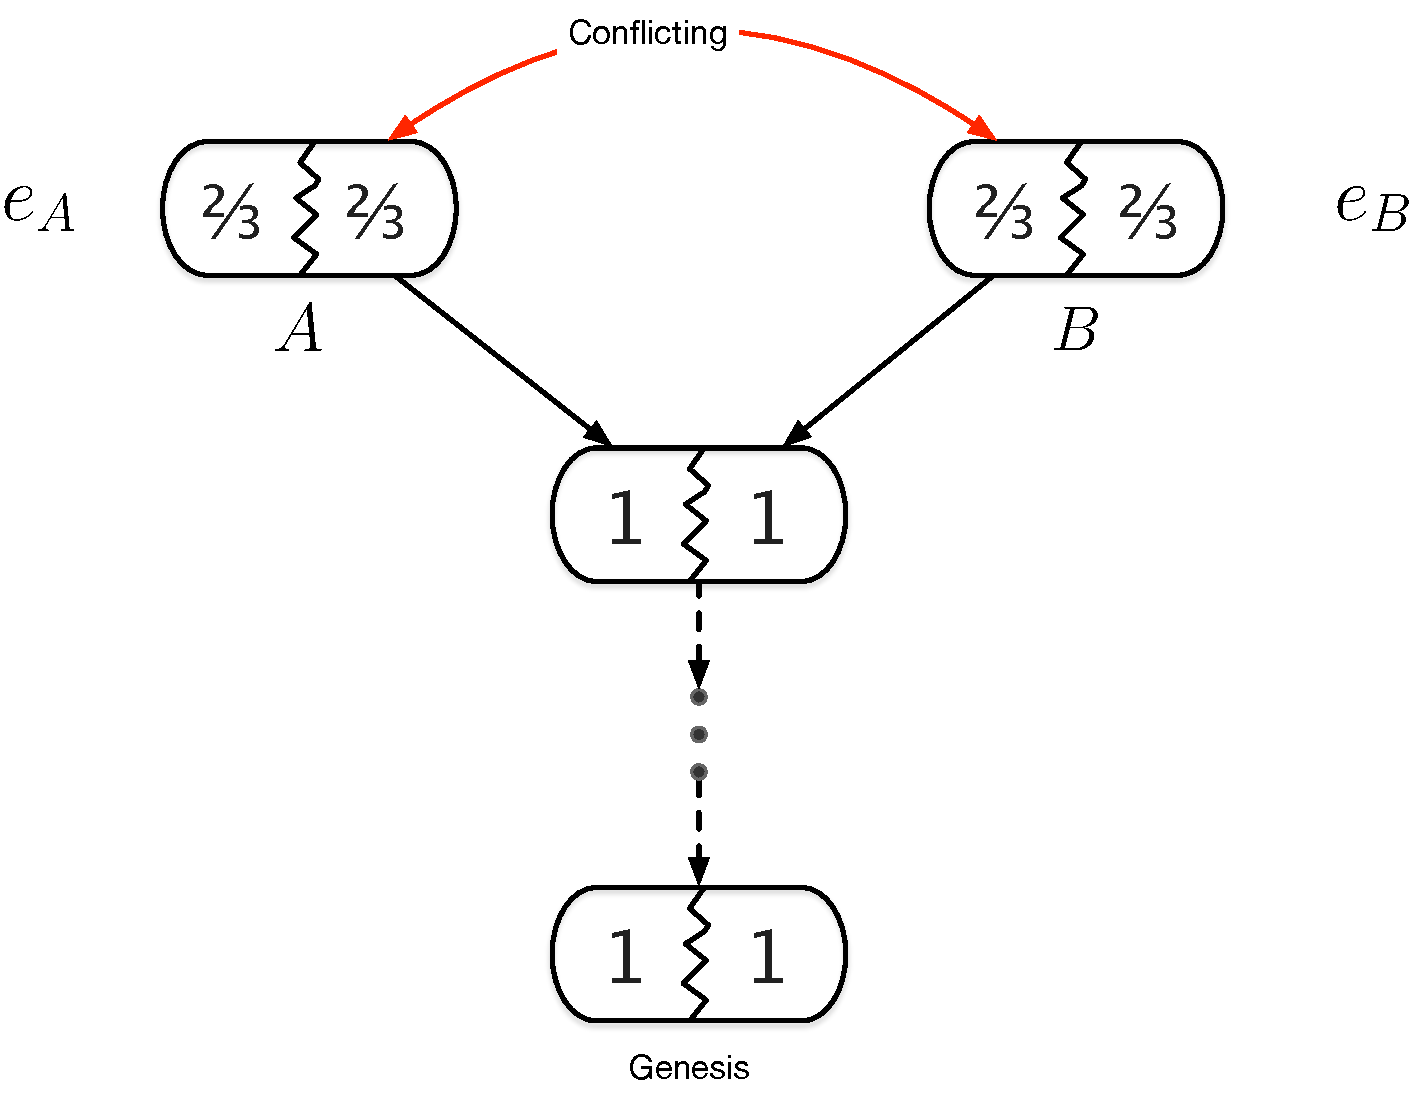
\includegraphics[width=2.5in]{Theorem1a.pdf}
	\caption{$\epoch_A = \epoch_B$}
	\label{fig:2a}	
	\end{subfigure}
	
\begin{subfigure}[b]{0.45\textwidth}
   \centering
   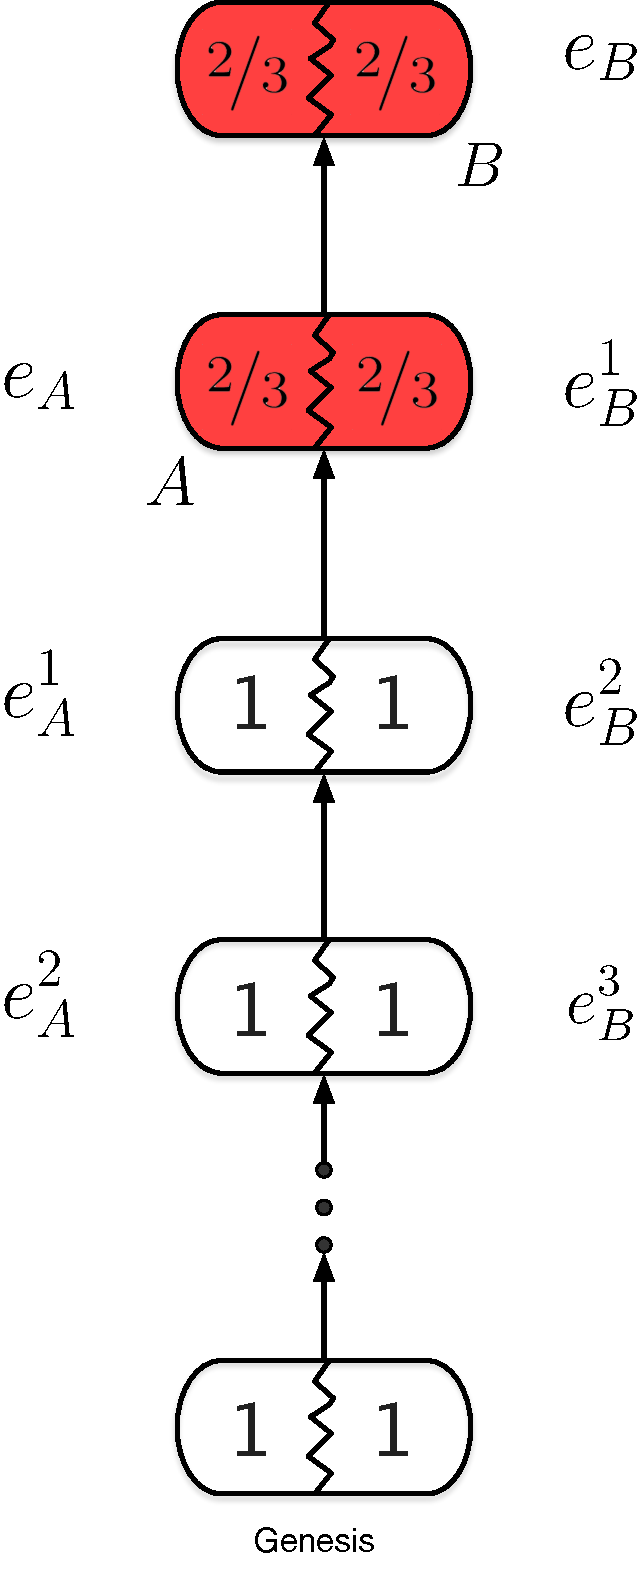
\includegraphics[height=2.7in]{Theorem1b.pdf}
	\caption{$\epoch_B^i = \epoch_A < \epoch_B$}
	\label{fig:2b}	
	\end{subfigure} \hspace{0.05\textwidth} 	 \begin{subfigure}[b]{0.45\textwidth}
   \centering
   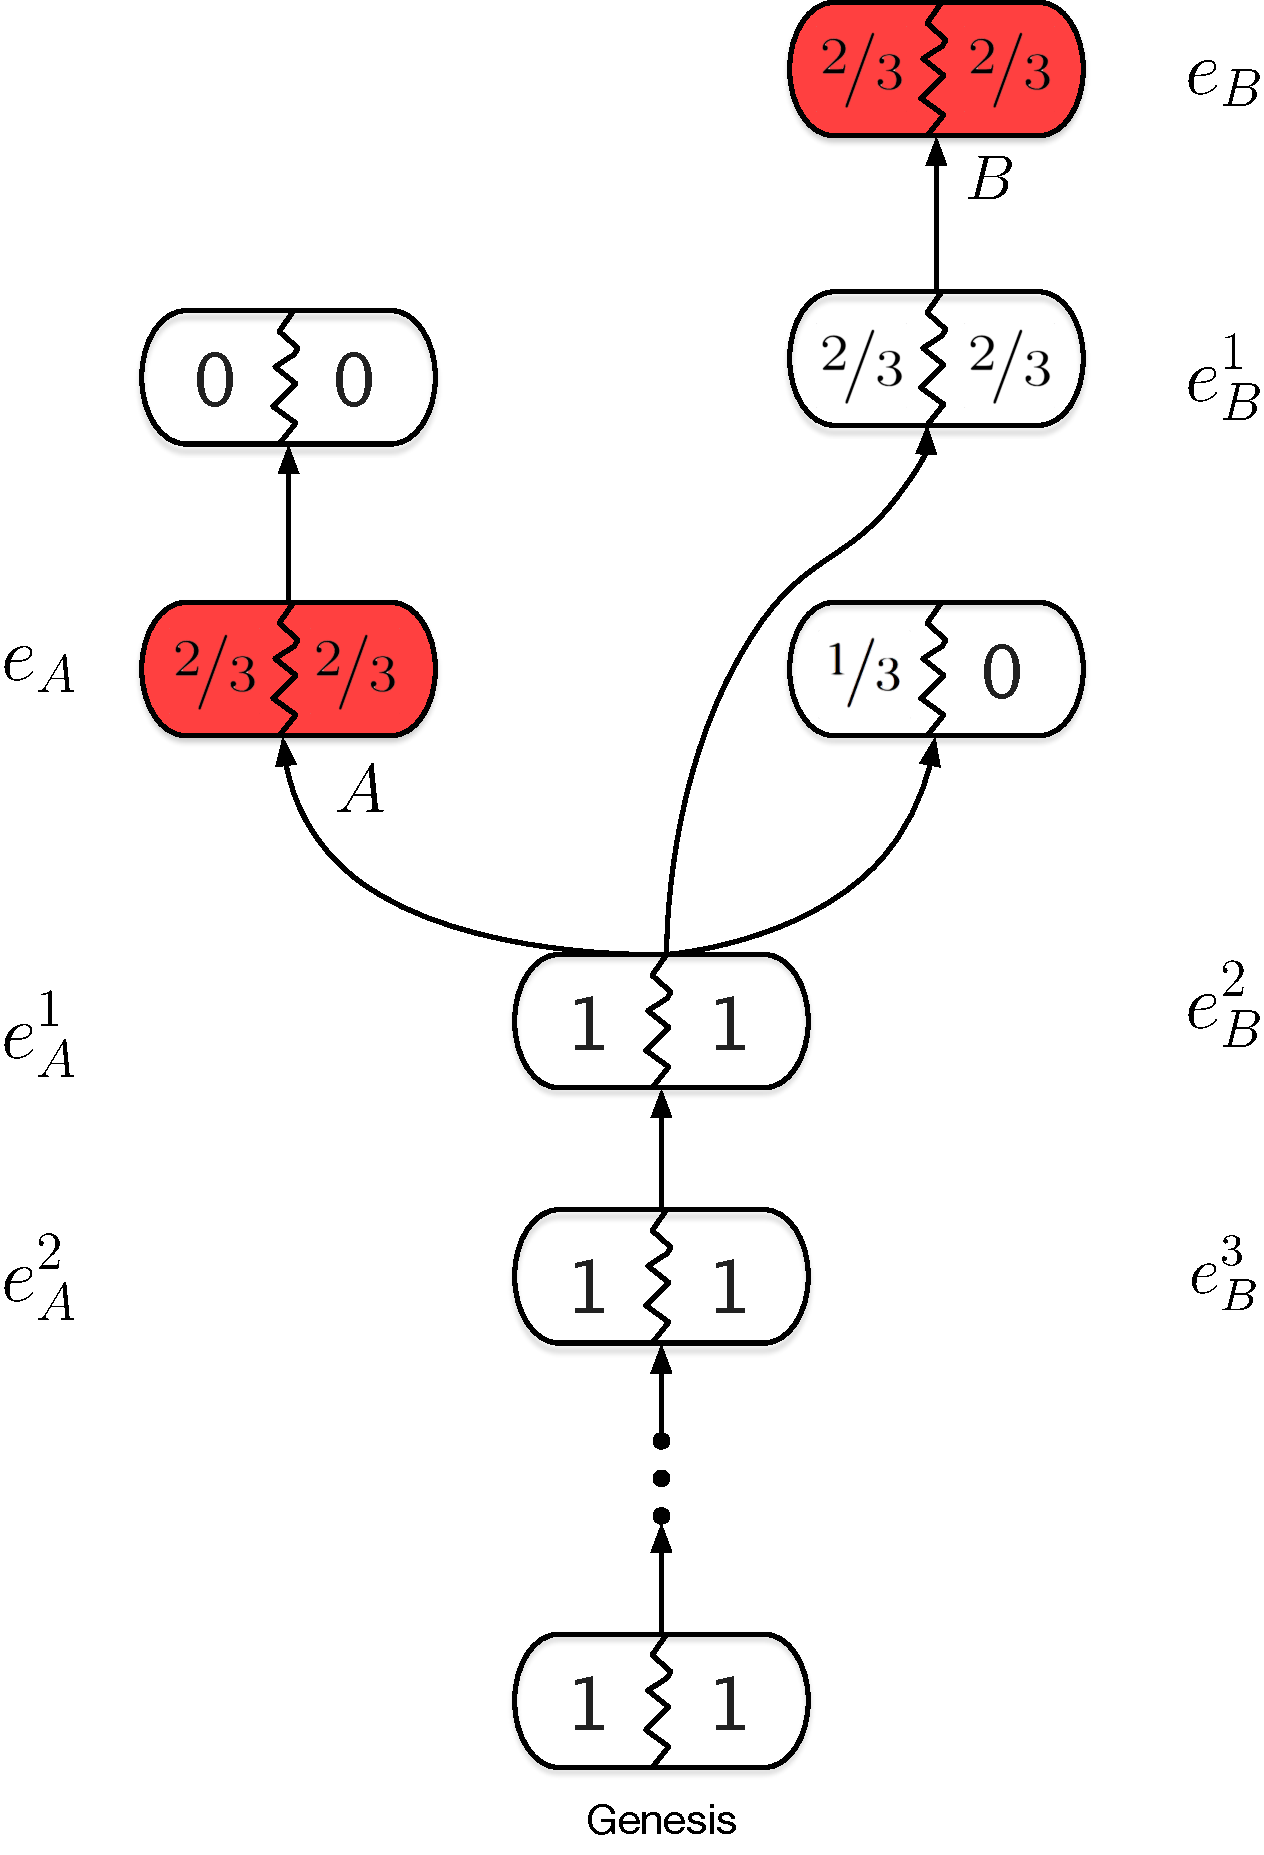
\includegraphics[width=2.7in]{Theorem1c.pdf}
	\caption{$\epoch_B^i < \epoch_A < \epoch_B$}
	\label{fig:2c}	
	\end{subfigure}

\caption{Illustrating the three scenarios in Theorem \ref{theorem:safety}.  Each pill represents a checkpoint.  In each pill, the left number is the proportion of validators who prepared that checkpoint, and the right number is the proportion of validators who committed that checkpoint.  Red pills are conflicting checkpoints.}
\label{fig:conflicting_checkpoints}
\end{figure}


\begin{theorem}[Plausible Liveness]
\label{theorem:liveness}
Regardless of what previous events took place, if $\geq \frac{2}{3}$ of validators never commit to an Unjustified block, a new checkpoint can be finalized without violating any Commandment.
%It is always possible for $\frac{2}{3}$ of honest validators to finalize a new checkpoint, .

\begin{proof}
Suppose all validators have sent some sequence of prepare and commit messages. Let $\hash_j$ at epoch $\epoch_j$ be the highest-epoch Justified checkpoint.  From the premise, $\geq \frac{2}{3}$ of validators have not committed to any epoch after $\epoch_j$.  Hence, Commandment \textbf{II} doesn't stop these validators from preparing any checkpoint $\hash$ at epoch $\epoch$ where $\epoch > \epoch_j$ and then committing $\hash$.  More concretely, these validators will always be able to publish $\langle \msgPREPARE, \hash_j, \epoch_j, \hash, \epoch \rangle$ and then publish $\langle \msgCOMMIT, \hash, \epoch \rangle$ without violating any Commandment.

% and let $n \ge \epoch_j$ be the highest epoch prepared by any honest validator. Honest validators have not committed on any block which is not Justified. 
\end{proof}

\end{theorem}


\section{Enabling Dynamic Validator Sets}
\label{sect:join_and_leave}

The set of validators needs to be able to change.  New validators must be able to join, and existing validators must be able to leave.  To accomplish this, we define a variable in the state called the \textit{dynasty counter}. \todo{We don't actually need this in the state.  It can be computed by each validator.} When a would-be valdiator's deposit message is included in dynasty $d$, then the validator will be \textit{inducted} at the start of dynasty $d+2$.  We call $d+2$ this validator's \textit{start dynasty}.


The dynasty counter increments if and only if there's been a \emph{perfectly finalized checkpoint}.  We define checkpoint $C_n$ as ``perfectly finalized'' if and only if during epoch $n-1$ every validator prepares $C_{n-1} \to C_{n}$ and commits $C_{n}$.  For example, checkpoint $C_3$ (a.k.a., $b_{199}$) is perfectly finalized if during epoch $2$, blocks $200 \ldots 299$ (before block $300$), \emph{all} validators prepare $b_{99} \to b_{199}$ \emph{and} commit $b_{199}$.

We define a growing sequence of the perfectly finalized checkpoints $\mathbf{P}$ starting simply as, $\mathbf{P} = \left( \Genesisblock \right)$.  Then, anytime a checkpoint is perfectly finalized, we append that checkpoint to sequence $\mathbf{P}$.  So if checkpoints $C_2, C_5, C_6, C_9$ are perfectly finalized, $\mathbf{P}$ becomes, $\mathbf{P} = \left( \Genesisblock, C_2, C_5, C_6, C_9 \right)$, and so on for future perfectly finalized checkpoints.  From the list of perfectly finalized checkpoints, we can compute the dynasty counter, $d \equiv | \mathbf{P} |$, and $\mathcal{D}(k)$ (where $k \in \left[1, |\mathbf{P}| - 1\right]$) as the set of checkpoints within dynasty $k$,
     
\begin{equation}
    \mathcal{D}(k) \equiv \begin{cases}
     \left\{ c \in \mathbf{C} : \mathbf{P}_k < c \right\} \qquad \qquad \qquad \!\! \textnormal{if $k = |\mathbf{P}| - 1$,} \\
         \left\{ c \in \mathbf{C} : \mathbf{P}_k < c \leq \mathbf{P}_{k+1} \right\} \qquad \textnormal{otherwise.} \\
     \end{cases}
\end{equation}

So using the example above, $\mathcal{D}(1) = \{ C_1, C_2 \}$,  $\mathcal{D}(2) = \{C_3, C_4, C_5\}$ and $\mathcal{D}(2) = \left\{ C_6 \right\}$, $\mathcal{D}(3) = \{ C_7, C_8, C_9\}$, etc.




To leave the validator set, the validator must send a ``withdraw'' message. If their withdraw message gets included during dynasty $d$, the validator similarly leaves the validator set at the start of dynasty $d+2$; we call $d+2$ the validator's \textit{end dynasty}.  At the start of the end dynasty, the validator's deposit is locked for a long period of time, the \textit{withdrawal delay}, (think ``four months'') before the deposit can be withdrawn.  If, during the withdrawal delay, the validator violates any Commandment, the deposit is forfeited.


\begin{equation}
    \mathcal{V}(k) = \left\{ \textnormal{validator set for dynasty $k$.  The accepted validators for checkpoints $\mathcal{D}(k)$.}\right\} \; .
\end{equation}


Which leads to the pleasing relations, $\mathbf{P} \subseteq \mathbf{F} \subseteq \mathbf{J} \subseteq \mathbf{C} \subset \mathbf{B}$ and $\mathcal{D}(k) \subseteq \mathbf{C} \ \ \forall k$.

\textbf{Revised requirement for accepting a prepare message (\figref{fig:msgPREPARE})}:
\begin{enumerate}
\item[5b.] The signing validator must be a member of the validator set for a specified dynasty.
\end{enumerate}


\textbf{Revised requirement for accepting a commit message (\figref{fig:msgCOMMIT})}:
\begin{enumerate}
\item[3b.] The signing validator must be a member of the validator set for a specified dynasty.
\end{enumerate}


For a checkpoint to be Justified, it must be prepared by a set of validators which contains (i) at least $\frac{2}{3}$ of the current dynasty and (ii) at least $\frac{2}{3}$ of validators comprising the previous dynasty. Finalization works the same. The current and previous dynasties will usually greatly overlap; but if the two validator sets substantially differ, this ``stitching'' mechanism mitigates the risk of a finality reversion or other failure can happen because different messages are signed by different validator sets and so equivocation is avoided.

We can write this mathematically by rewriting \eqref{eq:firstJandF} to become,
\begin{equation}
\begin{split}
    \mathbf{J} &= \left( c \in \mathbf{C} : \min\left[ \textnormal{valid\_prepares}(c,d-1), \textnormal{valid\_prepares}(c,d) \right] \geq \nicefrac{2}{3} \right) \\
    \mathbf{F} &= \left( j \in \mathbf{J} \,: \min\left[\textnormal{valid\_commits}(j,d-1), \textnormal{valid\_commits}(j,d) \right] \geq \nicefrac{2}{3} \right)\; ,
\end{split}
\label{eq:secondJandF}
\end{equation}
where $d$ is the current dynasty index.


\begin{figure}[h!tb]
\centering
\includegraphics[width=4in]{validator_set_misalignment.png}
%
\includegraphics[width=4in]{cs.pdf}
\caption{Without the validator set stitching mechanism, it's possible for two conflicting checkpoints to be Finalized with no validators slashed}
\label{fig:dynamic2}
\end{figure}

\TODO{not happy with this notation yet.}


\subsection{Long Range Attacks}
Note that the withdrawal delay introduces a synchronicity assumption \textit{between validators and clients}. Because validators can withdraw their deposits after the withdrawal delay, there is an attack where a coalition of validators which had more than $\frac{2}{3}$ of deposits \textit{long ago in the past} withdraws their deposits, and then uses their historical deposits to finalize a new chain that conflicts with the original chain without fear of getting slashed.  Despite violating slashing conditions to make a chain split, because the attacker has already withdrawn on both chains they do not lose any money. This is called the \textit{long-range atack}.

\begin{figure}[h!tb]
\centering
\includegraphics[width=3in]{LongRangeAttacks.png}
%
\includegraphics[width=3in]{cs.pdf}
\caption{Illustrating the long-range attack.}
\label{fig:dynamic3}
\end{figure}

We solve this problem by simply having clients not accept a Finalized checkpoint that conflicts with Finalized checkpoints that they already know about. Suppose that clients can be relied on to log on at least once every $\delta$ days, and the withdrawal delay is $W$. Suppose attackers send one Finalized checkpoint at time $0$, and then another right after. In the worst case, the first checkpoint arrives at all clients at time $0$, and that the second reaches a client at time $\delta$. The client will then know of the fraud, and will be able to create and publish an evidence transaction. We then add a consensus rule that requires clients to reject chains that do not include evidence transactions that the client has known about for time $\delta$. Hence, clients will not accept a chain that has not included the evidence transaction within time $2 * \delta$. So if $W > 2 * \delta$ then slashing conditions are enforcible.

In practice, this means that if the withdrawal delay is four months, then clients will need to log on at least once every two months to avoid accepting bad chains for which attackers cannot be penalized. \todo{convert this into a lemma/theorem.}

\section{Recovering from Castastrophic Crashes}
\label{sect:leak}

Suppose that $>\frac{1}{3}$ of validators crash-fail at the same time---i.e, they are no longer connected to the network due to a network partition, computer failure, or are malicious actors. Then, no later checkpoint will be able to get Finalized.

We can recover from this by instituting a ``leak'' which dissipates the deposits of validators that do not prepare or commit, until eventually their deposit sizes decrease low enough that the validators that \textit{are} preparing and committing are a $\frac{2}{3}$ supermajority. The simplest possible formula is something like ``validators with deposit size $D$ lose $D * p$ in every epoch in which they do not prepare and commit'', though to resolve catastrophic crashes more quickly a formula which increases the rate of dissipation in the event of a long streak of non-Finalized blocks may be optimal.

The dissipated portion of deposits can either be burned or simply forcibly withdrawn and immediately refunded to the validator; which of the two strategies to use, or what combination, is an economic incentive concern and thus outside the scope of this paper.

Note that this does introduce the possibility of two conflicting checkpoints being Finalized, with validators only losing money on one of the two checkpoints as seen in \figref{fig:commitsync}.

\begin{figure}[h!tb]
\centering
\includegraphics[width=4in]{CommitsSync.png}
\caption{The checkpoint on the left can be Finalized immediately. The checkpoint on the right can be Finalized after some time, once offline validator deposits sufficiently dissipate.}
\label{fig:commitsync}
\end{figure}

If the goal is simply to achieve maximally close to 50\% fault tolerance, then clients should simply favor the Finalized checkpoint that they received earlier. However, if clients are also interested in defeating 51\% censorship attacks, then they may want to at least sometimes choose the minority chain. All forms of ``51\% attacks'' can thus be resolved fairly cleanly via ``user-activated soft forks'' that reject what would normally be the dominant chain. Particularly, note that finalizing even one block on the dominant chain precludes the attacking validators from preparing on the minority chain because of Commandment II, at least until their balances decrease to the point where the minority can commit, so such a fork would also serve the function of costing the majority attacker a very large portion of their deposits.

\section{Conclusions}

This introduces the basic workings of Casper the Friendly Finality Gadget's prepare and commit mechanism and fork choice rule, in the context of Byzantine fault tolerance analysis. Separate papers will serve the role of explaining and analyzing incentives inside of Casper, and the different ways that they can be parametrized and the consequences of these paramtrizations.

\textbf{Future Work.} \todo{fill me in}

\textbf{Acknowledgements.} We thank Virgil Griffith for review.

\bibliographystyle{naturemag}
\bibliography{ethereum}
%\section{References}
%\bibliographystyle{plain}
%\bibliography{ethereum}
%\thebibliography

\appendix
\clearpage
\section{Unused text}

\todo{This is where text goes that for which a home hasn't been found yet.  If no home is found, it will be deleted.}



We define an \textit{epoch} as a range of 100 blocks (e.g., blocks 600...699 are epoch 6), and a \textit{checkpoint} of an epoch is the final block in that epoch. 

The proposal mechanism will initially be the existing Ethereum proof of work chain, making the first version of Casper a \textit{hybrid PoW/PoS algorithm} that relies on proof of work for liveness but not safety, but in future versions the proposal mechanism can be substituted with something else.



for the same \epoch and \hash as in \eqref{eq:msgPREPARE}.  The $\hash$ is the block hash of the block at the start of the epoch.  A hash $\hash$ being justified entails that all fresh (non-finalized) ancestor blocks are also justified.  A hash $\hash$ being finalized entails that all ancestor blocks are also finalized, regardless of whether they were previously fresh or justified.  An ``ideal execution'' of the protocol is one where, at the start of every epoch, every validator Prepares and Commits the first blockhash of each epoch, specifying the same $\epochsource$ and $\hashsource$.

In the Casper protocol, there exists a set of validators, and in each \textit{epoch} (see below) validators may send two kinds of messages: $$[PREPARE, epoch, hash, epoch_{source}, hash_{source}]$$ and $$[COMMIT, epoch, hash]$$


If, during an epoch $e$, for some specific ancestry hash $h$, for any specific ($epoch_{source}, hash_{source}$ pair), there exist $\frac{2}{3}$ prepares of the form $$[PREPARE, e, h, epoch_{source}, hash_{source}]$$, then $h$ is considered \textit{justified}. If $\frac{2}{3}$ commits are sent of the form $$[COMMIT, e, h]$$ then $h$ is considered \textit{finalized}.


During epoch $n$, validators are expected to send prepare and commit messages with $\epoch = n$ and $h$ equal to a checkpoint of epoch $n$. Prepare messages may specify as \hashsource a checkpoint for any previous epoch (preferably the preceding checkpoint) of \hash, and which is \textit{justified} (see below), and the \epochsource is expected to be the epoch of that checkpoint.


Honest validators will never violate slashing conditions, so this implies the usual Byzantine fault tolerance safety property, but expressing this in terms of slashing conditions means that we are actually proving a stronger claim: if two conflicting checkpoints get finalized, then at least $\frac{1}{3}$ of validators were malicious, \textit{and we know whom to blame, and so we can maximally penalize them in order to make such faults expensive}.


This simplifies our finalty mechanism because it allows it to be expressed as a fork choice rule where the ``score'' of a block only depends on the block and its children, putting it into a similar category as more traditional PoW-based fork choice rules such as the longest chain rule and GHOST\cite{sompolinsky2013accelerating}.

Unlike GHOST, however, this fork choice rule is also \textit{finality-bearing}: there exists a ``finality'' mechanism that has the property that (i) the fork choice rule always prefers Finalized blocks over non-Finalized blocks, and

\begin{figure}[h!tb]
\centering
    \includegraphics[width=3in]{prepares_commits.png}
%    
\includegraphics[width=5.5in]{cs.pdf}
    \caption{Illustrating prepares, commits and checkpoints. Arrows represent \textit{dependency} (e.g., a commit depends on there being $\frac{2}{3}$ existing prepares).}
    \label{fig:prepares_and_commits}
\end{figure}


\begin{enumerate}
\item Start with HEAD equal to the genesis of the chain.
\item Select the descendant checkpoint of HEAD with the most commits (only Justified checkpoints are admissible)
\item Repeat (2) until no descendant with commits exists.
\item Choose the longest proof of work chain from there.
\end{enumerate}



\section{Notes to Authors}
\subsection{Questions}
\begin{itemize}
\item True/False: The Dynasty counter increments iff there's been a finalization?
\end{itemize}


\subsection{Notes on Suggested Terminology}
\begin{itemize}
\item parent $\rightarrow$ predecessor.
\item child $\rightarrow$ successor (unless want to emphasize there can be multiple candidate successors)
\item ancestors $\rightarrow$ lineage
\item to refer to the set of $\{$ predecessor, successor $\}$ $\rightarrow$ adjacent
\end{itemize}


\subsection{Todo}
\begin{itemize}
\item \todo{Reference the various Figures within the text so we more easily know what goes with what.}
\item \todo{fill me in}
\end{itemize}


In the other way...



%%%%%%%%%%%%%%%%%%%%%%%%%%%%%%%%%%%%%%%%%%%%%%%%%%%%%%


\end{document}
    